%!TEX root = ../template.tex

\chapter{3.	Approach to Elaboration Phase}
\label{cha:approach_to_elaboration_phase}

This chapter will discuss and present an overview of the elaboration phase. It will describe in fine detail the objective and contributions of this dissertation and how it is planned to archive those goals. It should provide a detailed and clear roadmap to implement a system that will comply with all the objectives goals and requirements of this thesis.

In section \ref{sec:refinement_of_objectives_and_contributions} the objectives and contributions are refined and exposed clearly and matched against the related work performed and discussed in chapter \ref{cha:related_work}. It will discuss the scenario and environment under where the system should fall.

Section \ref{sec:system_model_approach} its presented the general system model of the contributions and objectives. It describes the model of the planned system implementation.

The architecture and implementation details of the solution are present in section \ref{sec:planned_architecture_and_implementation}. This section will dive in more detail on how and with what technologies the system will be implemented with.

Having discussed the solution implementation, section \ref{sec:planned_testbench_environments} explains how and where it is planned to test the system, whereas section \ref{sec:relevant_evaluation_criteria} will complement it with what metrics will be gathered and how they will be compared with each other.

\section{Refinement of Objectives and Contributions} % (fold)
\label{sec:refinement_of_objectives_and_contributions}

To achieve the objectives proposed in chapter \ref{cha:introduction}, we will work under a specific scenario, that can be described using an adversary model and some system assumptions. The goal of creating a secure in-memory storage based on secure hardware technologies must have a well defined scope and be thorough across that same scope. The system adversary/threat model and assumptions will be described in sections \ref{ssec:adversary_model} and \ref{ssec:system_assumptions} respectively.

\subsection{Adversary Model}
\label{ssec:adversary_model}

The threat model basis for the system will lie on the gls{SGX}'s model. We will assume their model and protection overview stated in \gls{SGX}'s paper \cite{sgx:7}.

\textit{SGX prevents all other software from accessing the code and data located inside an enclave including system software and access from other enclaves. Attempts to modify an enclave’s contents are detected and either prevented or execution is aborted}, \cite{sgx:7} which falls in the following adversary model:

\textbf{Malicious applications or code:} The system protects its data from an attacker capable of compromising the system through another application installed on the same system. This includes code from the \gls{OS} hypervisor or any other code in the machine.

\textbf{Honest but Curious (or Malicious System Administrator):} The system must be able to protect from an attacker with root access to the machine. Data deployed on the cloud should only be read by the user and not by any cloud system administrators with ability to examine and modify the system.

\textbf{Network Attacks:} All communication to and from the system should be secure. We assume attacker capable of intercepting, replaying and tamper with messages in the transport layer. 

\textbf{File system and memory access attacks:} All sensitive data residing outside protected memory should be encrypted. An attacker can access the physical disks and hardware without the data being exposed.

\subsection{System Assumptions}
\label{ssec:system_assumptions}

The system planned has certain assumptions and aspects that are considered to be out of scope for this dissertation:

\begin{itemize}
	\item \textbf{Trusted Client} - The client side is assumed to be completely trusted and correct.
	\item \gls{DoS} and \gls{DDoS} attacks are out of scope.
	\item Side Channel Attacks - It is out of scope any side channel attacks or any related attack not present in \gls{SGX}'s threat model.
	\item Physical and Hardware attacks - It is out of scope any physical or hardware attacks or any related attack not present in the \gls{SGX} threat model.
	\item \gls{SGX} limitations or security issues - Any limitation or security issues known to the technology, either present on the \gls{SGX}'s paper and/or explain in section \ref{ssec:circumvention_of_sgx_limitations}.
\end{itemize}

\section{System Model Approach} % (fold)
\label{sec:system_model_approach}

System model approach

\section{Planned Architecture and Implementation} % (fold)
\label{sec:planned_architecture_and_implementation}

Planned architecture and implementation

\section{Planned Testbench Environments} % (fold)
\label{sec:planned_testbench_environments}

Planned testbench environments

\section{Relevant Evaluation Criteria} % (fold)
\label{sec:relevant_evaluation_criteria}

\begin{figure}[htbp]
  \centering
  \subcaptionbox{One sub-figure\label{fig:leftsubfig}}%
    {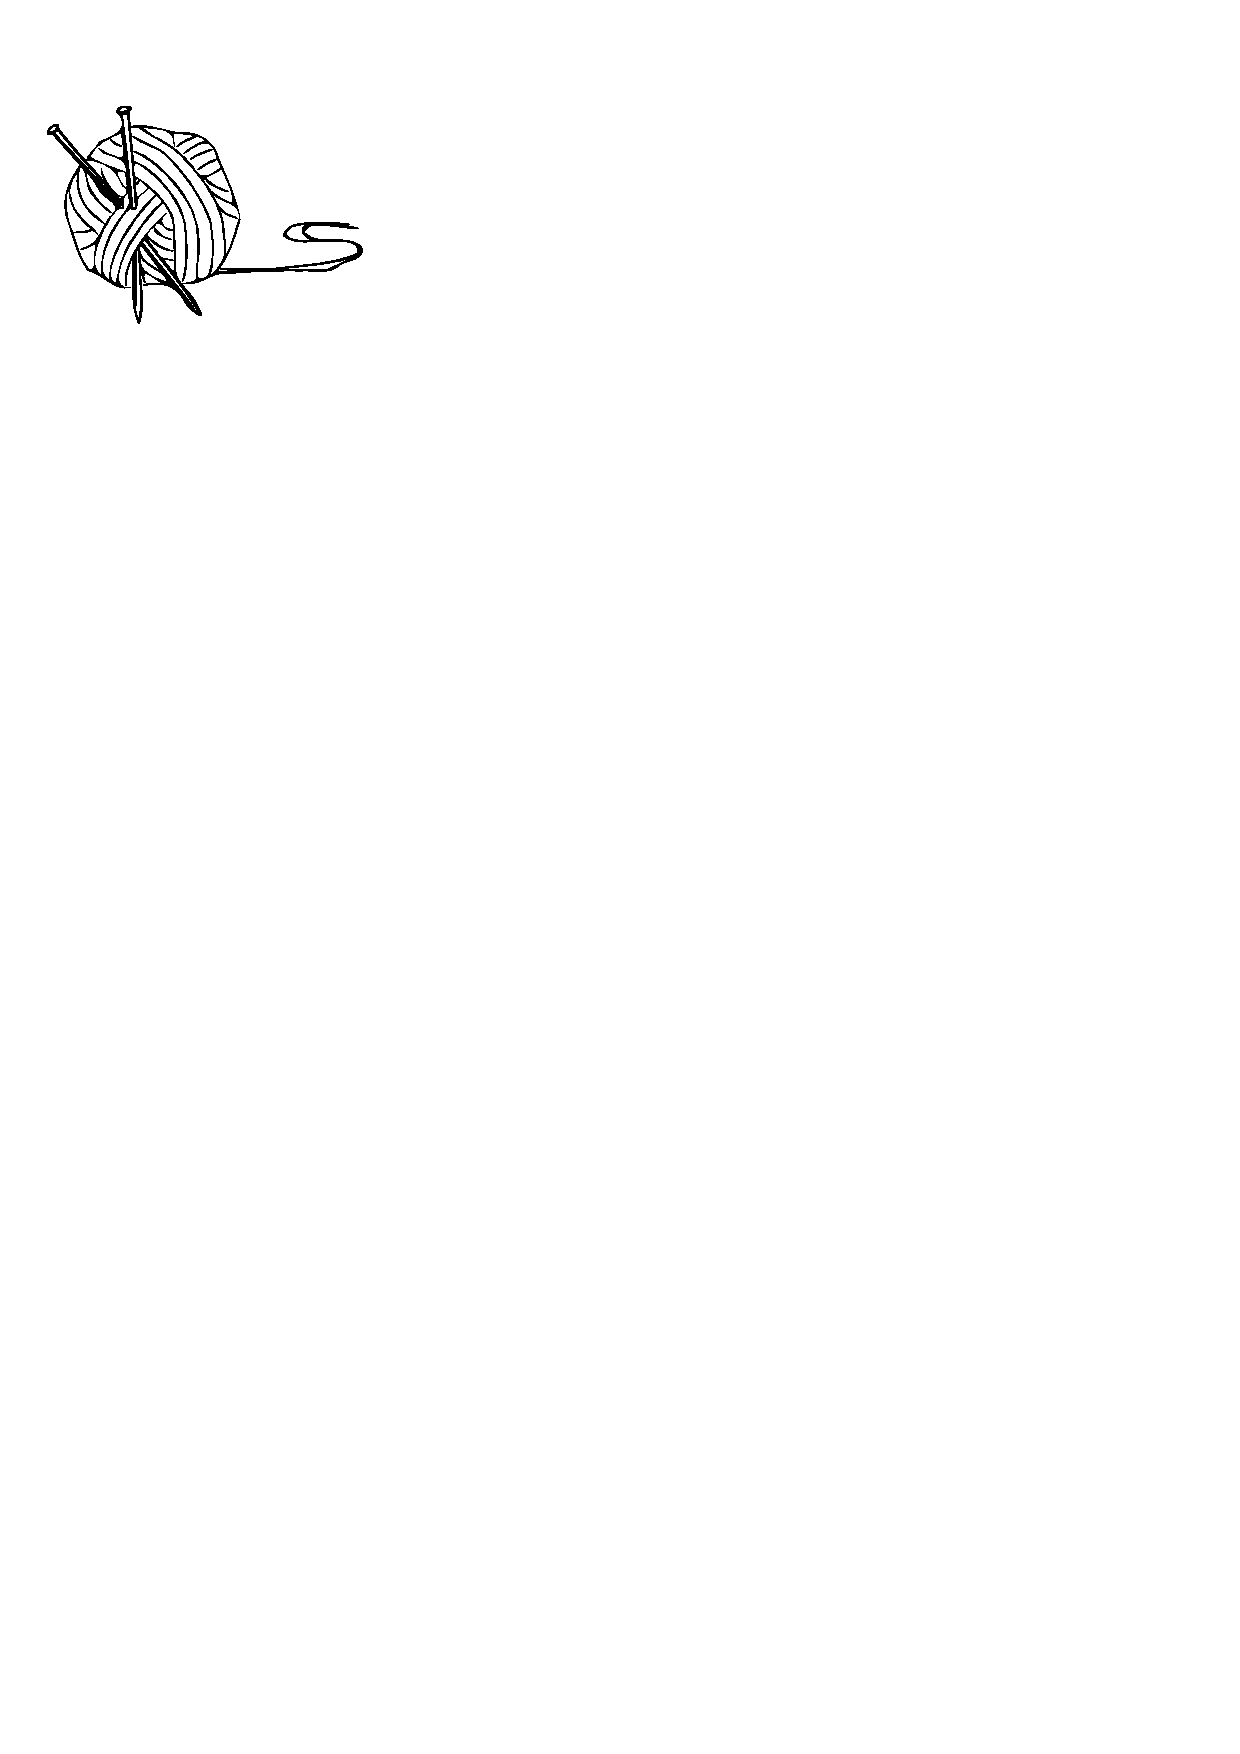
\includegraphics[width=0.5\linewidth]{knitting-vectorial}}%
  \subcaptionbox{Another sub-figure\label{fig:rightsubfig}}%
    {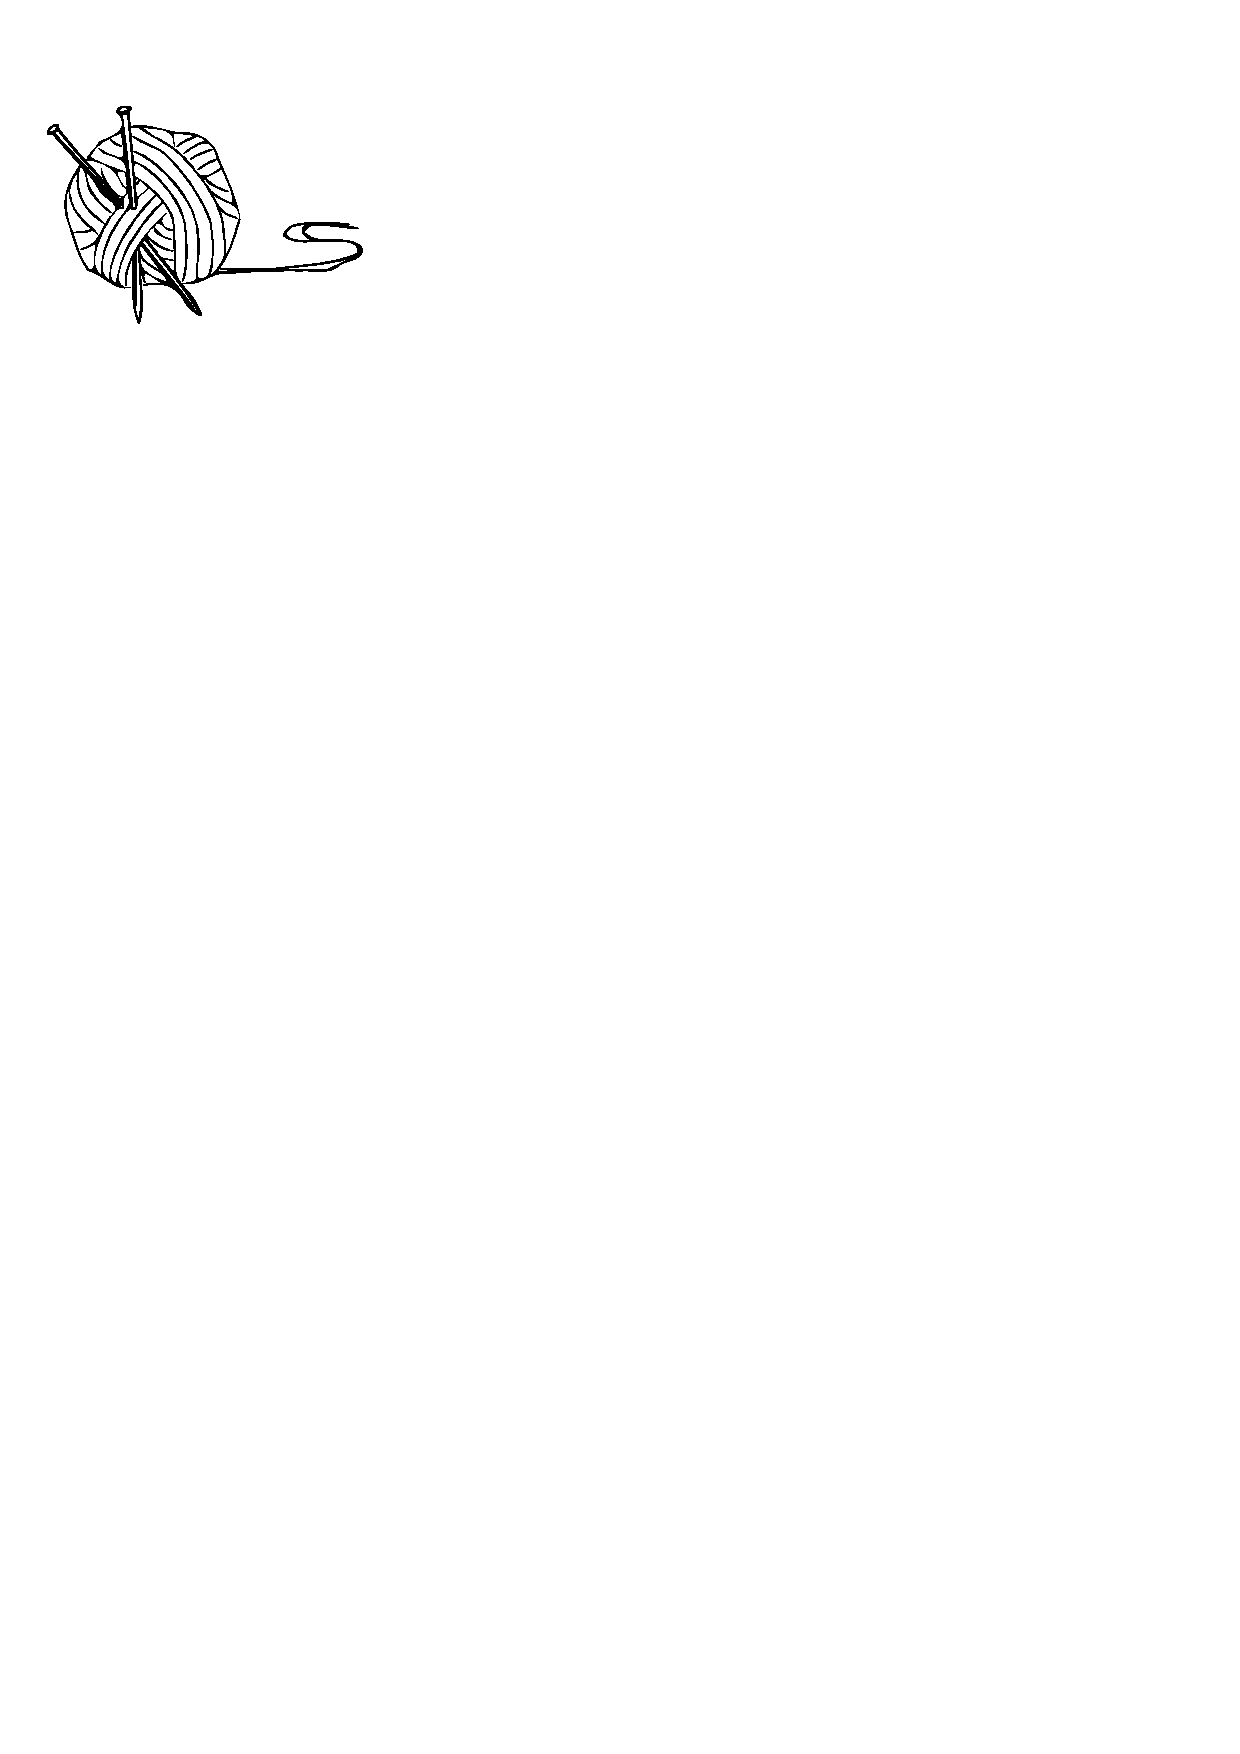
\includegraphics[width=0.5\linewidth]{knitting-vectorial}}%
  \caption{A figure with two sub-figures!}
  \label{fig:fig2subfig}
\end{figure}

\textbf{And this is a small text that references the Figure~\ref{fig:fig2subfig} and its Subfigures~\ref{fig:leftsubfig} and~\ref{fig:rightsubfig}.}

Chapter 3